\subsection{De la physique au calcul informatique}
Pour pouvoir faire une simulation de réservoir, tout commence par un physicien qui modélise un écoulement de fluide en milieu poreux.
%
La plupart de ces modèles sont basés sur trois équations physiques : la conservation de la masse, la loi des gaz parfaits et la loi de Darcy.
%
Puis le réservoir est discrétisé en cellules en utilisant la méthode des volumes finis.
%
Pour chaque cellule du réservoir, nous obtenons une équation non-linéaire par variables primaires (ex.: pression, saturation en huile, ...).
%
Pour résoudre le système d'équations non-linéaires nous utilisons la méthode NewtonRaphson.
%
Cette méthode est itérative, nous démarrons avec une valeur initiale $X_0$ suffisamment proche de la solution $X_n$ qui satisfait $F(X_n) = 0$.
%
La méthode NewtonRaphson nous garantit que chaque itération nous rapproche du minimum local sous condition que le hessien soit défini positif.

%   (-_-)   %
\begin{figure}[!h]
  \centering
  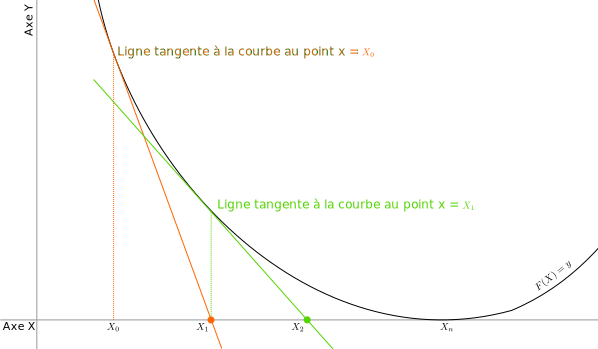
\includegraphics[width=0.8\textwidth]{newton}
  \caption{Exemple de deux étapes de Newton en une dimension.
    Chaque tangente correspond à une équation linéaire à résoudre.
    Nous recherchons $X_n$ et nous démarrons au point $X_0$.}
\label{fig:newton}
\end{figure}


L'exemple de la figure~\ref{fig:newton} n'est que dans une seule dimension, mais la même approche peut être utilisée quand on travaille avec un nombre arbitraire de dimensions.
%
Les équations linéaires de la simulation de réservoir peuvent être représentées sous la forme d'une matrice creuse très grande, nous reviendront sur la définition de creuse plus loin dans ce manuscrit.
%
Dans cette matrice, chaque ligne représente les interactions des éléments d'une cellule avec les éléments de son voisinage direct.
%
Donc, si nous prenons un cube 3D régulier, nous pouvons avoir jusqu'à sept interactions par lignes.
%
Chaque interaction est représentée sous la forme d'une petite matrice dense dont la taille correspond au nombre de variables physiques simulées.
%
Par la suite, un solveur de systèmes d'algèbre linéaire creux est utilisé.
%
Pour la simulation de réservoir, nous utilisons un FGMRES préconditionné parce que nos matrices ne sont pas symétriques et que le préconditionneur classique CPR ne correspond pas à un opérateur linéaire fixe au cours des itérations~\cite{cao2005parallel}.
